\chapter{取り扱うデータの条件}
科学的に事象を取り扱うための本書で扱うデータの条件は以下の通りである。
これらが無いならば、本書で扱える範囲を超えている。統計学者に相談した方が良い\footnote{最初から統計学者に相談した方が良い}。

\begin{itemize}
    \item 再現性 同じような条件であれば、同じような現象が生じるということである。
    \item 計測誤差  計測により生じた誤差(測定誤差)は揺らぎ(集団内での差)に比べて十分に小さい
    \item 無作為抽出 なるべく偏りなく母集団からデータを取得する%母集団の特徴を捉えるためのデータの収集方法
    \item 実験デザイン バイアスを小さくなるように計画を行う。
    \item 予測 データを集めると、データとモデルの予測に関して相違点が明らかになり、モデルの改訂が必要になる。この改訂に終わりはない。
\end{itemize}

%みたいものを見るための計測方法がランダムサンプリングである。

\begin{SMbox}{何を学ばなければならないか}
    \cite{box1976science}から引用しておく。
    \begin{quote}
        We may ask of Fisher \\
        Was he an applied statistician? \\
        Was he a mathematical statistician?  \\
        Was he a data analyst? \\
        Was he a designer of investigations?\\
        It is surely because he was all of these that he was much more than the sum of the parts. He provides an example we can seek to follow. 
    \end{quote}
    %Fisherみたくなるのは難しいので、実験デザインと
\end{SMbox}

\section{実験デザイン}
わたしが扱える範囲ではないので、他書を読んだ方が良い。
今後まとめたい。
\begin{SMbox}{あとでまとめたいTODO}

    'Pseudoreplication' problem‐接着したコドラートは何が悪いのか
 \url{http://www.mus-nh.city.osaka.jp/iso/argo/nl02/nl02-21-32.html}
\end{SMbox}

\section{無作為抽出されていない事による過誤}
対象を無作為に抽出できていない標本から、統計量を計算し、モデルの母数を推定したとする。
このモデルでは、本来設定した母集団に関する予測には誤りが多くなる。
例えば、17歳の日本人男性の身長を母集団に指定したのに、17歳のバスケ部部員の身長を計測する。
その標本を元に、モデルの母数を推定し、母集団に関する推測を行う。
すると、その予測は母集団に関して十分なものではなくなる。
例えば、平均が大きくなりすぎたり、平均よりも小さな人の割合が予測と異なることが生じる。
%その標本を元に、想定していた母集団に関しての推測を行おうとする。
%そうしたとき、その予測は母集団に関して十分なものではなくなる。

やってはいけないとは言い切れないが、偏った集団を計測してしまった場合、
その解釈に一工夫が必要になる。


\subsection{Questionable Research Practice(QRP)}
以下ではやってはいけないことを紹介する。
国立研究開発法人 日本医療研究開発機構が出版している研究公正に関するヒヤリ・ハット集の
「7 研究データの信頼性、再現性等 」に詳しくまとめられている\footnote{\url{https://www.amed.go.jp/content/000064531.pdf}}。
% http://bunkei.ila.titech.ac.jp/sotsuronexcellence/class18_furui_kairi.pdf
\subsection{後付けの母集団かつ$p<\alpha$を満たす集団}
母集団Aを設定し、標本を抽出したものを標本aとする。標本aのデータはさまざまな要素から構成されているとする。例えば、ある会社に所属する人の、身長や年収、税金の支払い履歴、ローン残高、労働部署、高校時代の部活などであるとする。
この標本から、何らかの属性$A'$に当てはまるデータbを抽出したとする。
データbについて特定の統計モデルとの乖離するかを調べ、乖離していることをが判明したとする(乖離を定量的に調べる方法はなんでもいいが、$p<\alpha$だったと考えても良い)。
この結果から、属性$A'$に関わると考えられる母集団A'を再構成する。
そこから、母集団$A'$を特定のモデルで予測できないと結論づけることはできない。

まず、今集めた標本$a$は、母集団$A$から集めたものであり、母集団$A'$から集めたものではない。
よって、母集団$A'$から無作為抽出できていない。
また、標本aを無作為抽出したときに付随して得た、母集団$A'$の一部の偏った集団のデータである。
以上から、母集団$A'$に関する無作為抽出とはいえない。
図\ref{fig:conceptual_diagram_HARKing}には、概念図を示しておいた。

\subsubsection{後付けの母集団かつ$p<\alpha$を満たす集団}
$p<\alpha$であるという標本がデータから発見されたので、標本の特性を持つと思われる母集団を後付けし、その母集団から無作為抽出を行なったことにし、ある統計モデルとデータが乖離していたと言うストーリーを作ったとする。
%統計モデルが棄却されたというストーリーを作ったとする。
言い換えれば、後付けの母集団ならば、$p<\alpha$であるという論理を立てたとする。
実際には、後付けの母集団でありかつ$p<\alpha$という集団から作為抽出しているので\footnote{この場合でも無作為抽出できていると誤解してしまうが、後付けの母集団から無作為抽出できていない!}、本来の母集団については何もわからない。言い換えれば、母集団に関する拡大解釈が行われたことで、母集団に関しては何もわからないのに、推測を行なったと主張している\footnote{実際調査した母集団は母集団かつ$p<0.05$に対して、報告した母集団デカすぎんだろ...}。
母集団の特徴を知るには、無作為抽出を行い、推測を行う必要がある。

\begin{figure}
    \begin{center}
        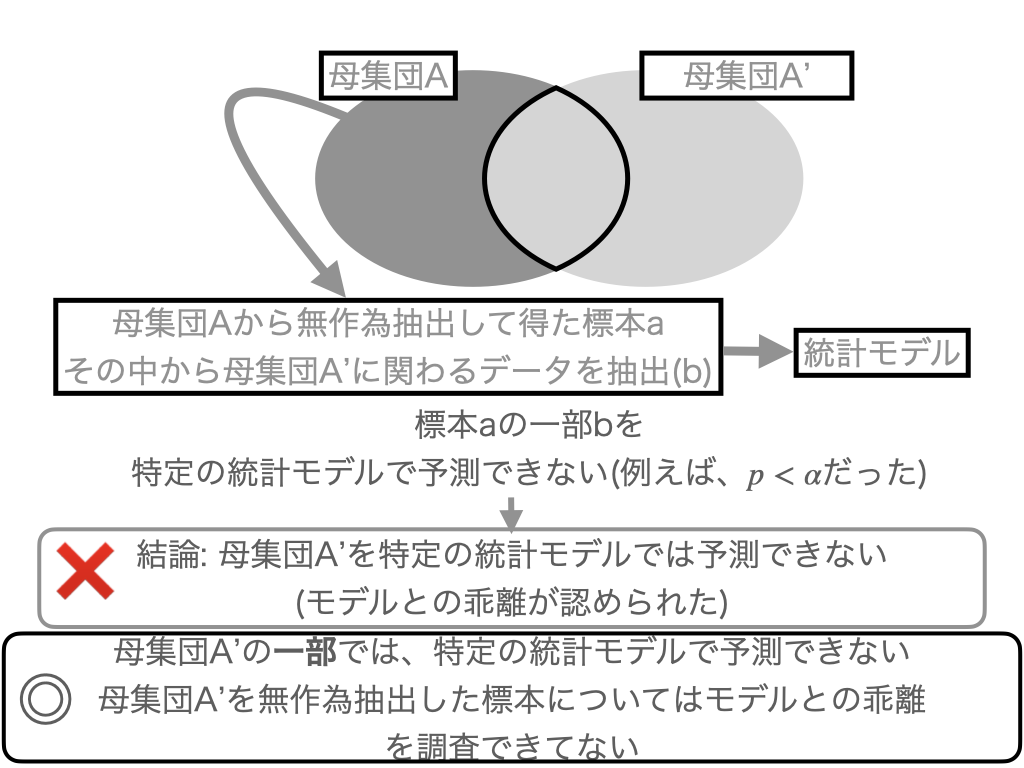
\includegraphics[width=15cm]{./image/01_/conceptual_diagram/conceptual_diagram.005.png}
        \caption{仮説ハッキングの概念図}
        \label{fig:conceptual_diagram_HARKing}
    \end{center}
\end{figure}
    

このような母集団に関する拡大解釈を仮説ハッキング($HARKing$(Hypothesizing After the Results are Known))といい、この操作により得たデータと仮説について、仮説が元からあったことにして、報告を行うと、研究不正となる\footnote{
    HARKingは、再現性の問題という意見もある。
    \url{https://twitter.com/ykamit/status/1077716200845500416} 。この意見に私は同意する。母集団を無作為抽出していないことで、再現できないことが増えると考えられる。
}
\footnote{
    多重検定により、$p$値が低く推測されることが問題であるというものもある\cite{池田_功毅2016,中村_大輝2021sp20016}。部分的には同意できるが、私は十分理解できなかった。
}\footnote{
    Twitterでのアンケートでは、多くの人がHARkingをうまく理解できてないというTwitterでのアンケートもある。
    \url{https://twitter.com/biomedcircus/status/1088957697368690689}
}\footnote{
    探索的なデータ解析においては、帰無仮説の後付けが許されるという主張もある。この意見には同意できない。母集団について拡大解釈をすることは許されない。探索的データ解析により得られるのは、母集団かつ$p<\alpha$という集団が見つかったということのみ主張できる。
    これを元に、母集団に関する性質を言及してしまうのはおかしい。
    %母集団についての推測をしたと主張はできない。
}\footnote{
    HARKingについては、\cite{kerr1998harking}に詳しくまとめられている
}。

%https://twitter.com/Hiroshi12337131/status/1613560913889742849
% https://twitter.com/ykamit/status/1615162295986028546
% https://twitter.com/ykamit/status/1090791485312720896

\begin{SMbox}{HARKing}
    \begin{rightbubbles}{bubblegreen}{Yuki Kamitani}{./image/Twitter_logo_EPS/2021_Twitter_logo_blue.eps}
    データを操作してp値をいじる行為を不正と認識している人は多いが、HARKingが不正と思っている人は非常に少ない。私の周辺分野のシニア研究者で理解している人はほぼ皆無(問題を指摘すると一笑に付される)。研究の実践と論文フォーマットの齟齬やフェアプレー精神の問題(?)と理解している人がいた
        \begin{flushright} 
            \small	\url{https://twitter.com/ykamit/status/1077715969827528705}
        \end{flushright}    
    \end{rightbubbles}

    HARkingを理解するのは、難しい。無作為抽出したデータから、データを調べた後に、母集団を構成しているのだから、無作為抽出できていると考えてしまいがちになる。
\end{SMbox}
  

\subsection{$p<\alpha$になったら無作為抽出を終える}
$p$値がある値を下回ったときに、実験を終了するという操作を行なったとする。
統計モデルの予測と一致するように、母集団を選択したことになる。
この場合、無作為抽出した集団により、設定した母集団に関する性質を調べるという研究目的を達成できない。
「母集団かつ設定したモデルにおいて$p<\alpha$である」集団に関する調査を行なっていることになる。

調査を終えて、この標本についてモデルを使った予測ができないと主張できない。
この不正な操作をアステリスクシーキングという。


\subsection{標本平均がxxになったときに抽出を終える}
標本に対して計算できる平均値や分散が理想の(考えているモデル)と一致するまで無作為抽出を繰り返すまたは、一致したときに無作為抽出を終えると、無作為抽出したとは言いきれない。


\begin{SMbox}{計測したデータを報告しない}
    \begin{quote}
        日本製鉄は18日、東日本製鉄所君津地区(千葉県君津市)から有害物質が流出していた問題で、過去の水質測定データに不適切な扱いがあったと発表した。排出基準を超える有害物質が検出されたにもかかわらず、千葉県などに報告していない例があった。有害物質が基準を上回った際、再度測定して基準内に収まる結果を記録していたことも明らかにした。
        \ \ \\ \url{https://www.nikkei.com/article/DGXZQOUC186070Y2A810C2000000/}
    \end{quote}

    アンモニア化合物の漏洩が発生し、着色水の構外への流出が確認され、排水溝から取水したサンプルから、環境規制値を超えるシアンが検出される   \footnote{東日本製鉄所君津地区における着色水の構外への流出について \url{https://www.nipponsteel.com/common/secure/news/20220624_100.pdf}}。
    その後、シアン除去設備の能力増強などが行われる\footnote{\url{https://www.nipponsteel.com/common/secure/news/20220706_100.pdf}}。
    さらに、精査していくと、測定データについて不適切な取り扱いがあったことが判明した\footnote{\url{https://www.nipponsteel.com/common/secure/news/20220818_200.pdf}}。
    ここで、1日のうちに複数回の計測データが存在していたこと、関係機関へ報告していた数値より高い計測データが存在していたことが判明した。

    計測データが、予想や基準値よりも大きかったまたは小さかったから、データを削除してはいけない。
    計測手順を決定し、そして計測したデータは、全て報告しなければならない。

    データが恣意的に削除されているかどうかを判定することは非常に難しい。
    この例でも、データを持たない外部の人間が、不適切な報告が行われていることを判定できなかった。
    基準値を超えたデータについても記録が残っていたので、報告が適切に行われていないことが明らかになった。


    データがなければ、どのような行動を行うだろうか。
    例えば、保存されたサンプルを再度計測することになる。
    そのサンプルがなければ、なぜ基準値を超えた値が検出されたのかが徹底的にせいさされることになる。例えば、計測装置の利用手順のミスなどが検証される。
    ここで異常がなければ、通常のサンプリングが行われ、基準値を超えるデータが取得される頻度が、これまでよりも高いかを調べることになると考えられる。
    データがなければ、検証のコストが増えてしまうと考えられる。

    
    %川が赤くなっているという報告が上がったこともあり、調査が行われたようである\footnote{\url{https://news.yahoo.co.jp/articles/ea20d54623642b848960d93404aad6eba3ffae4a}}

\end{SMbox}

\section{Garbage in, garbage out}
以上のことを守っていないデータは、ゴミデータである。
ゴミデータを統計処理したならば、ゴミのような推論しか得られない。
言い換えれば、意味のある結果を返しにくくなったり、解釈が難しくなることがある。

\section{みにくいアヒルの子の定理}
特徴量の取り方
%https://atmarkit.itmedia.co.jp/ait/articles/2007/30/news024.html

\section{ノーフリーランチ定理}

\if 0
自分の言葉に書き換えよう
\begin{quote}
    もしアルゴリズムが、ある特定領域の問題において優れた性能を発揮しているのなら、それ以外の残り全ての問題群においては性能が低下する代償を支払う必要がある
    \url{https://atmarkit.itmedia.co.jp/ait/articles/2007/17/news020.html}    
\end{quote}
\fi 
